\section{Covariância e Coeficiente de Pearson}

\begin{frame}{Qual Problema de Ciência de Dados?}
    \begin{itemize}
        \item \textbf{Objetivo:} Mensurar o efeito de uma variável preditora $X$ na variável resposta $Y$.
        \item Em aulas anteriores, vimos abordagens baseadas em testes de hipóteses:
        \begin{itemize}
            \item Qual o efeito do hábito de fumar no peso dos bebês? $\implies$ \textbf{Negativo}.
            \item Qual o efeito de uma vacina na incidência de uma doença? $\implies$ \textbf{Ainda não sabemos}.
            \item Qual o efeito da escalação de um time no salário dos jogadores? $\implies$ \textbf{Sem significância estatística}.
        \end{itemize}
        \item \textbf{Nova Abordagem:} Responderemos a essas mesmas perguntas quantitativas via modelagem e regressão!
    \end{itemize}
    \vspace{0.4cm}
    \centering
    \Large{Variável Preditora ($X$) \quad $\longrightarrow$ \quad Variável Resposta ($Y$)}
\end{frame}

\begin{frame}{Caso Real: Veículos Híbridos}
    \begin{itemize}
        \item \textbf{Quais correlações seria interessante observar neste conjunto de dados?}
        \item \textbf{Quais relações seriam potencialmente causais?}
    \end{itemize}
    \vspace{0.2cm}
    \centering
    \footnotesize
    \begin{tabular}{lrrrrl}
    \toprule
    Modelo & Ano & Preço (mil USD) & Acc (s) & Consumo (mpg) & Classe \\
    \midrule
    Prius (1ª Ger) & 1997 & 24,51 & 7,46 & 41,26 & Compacto \\
    Tino & 2000 & 35,35 & 8,20 & 54,10 & Compacto \\
    Prius (2ª Ger) & 2000 & 26,83 & 7,97 & 45,23 & Compacto \\
    Insight & 2000 & 18,94 & 9,52 & 53,00 & Dois Lugares \\
    Civic (1ª Ger) & 2001 & 25,83 & 7,04 & 47,04 & Compacto \\
    \bottomrule
    \end{tabular}
\end{frame}

\begin{frame}{Correlação: Aceleração vs. Preço}
    \begin{columns}
        \begin{column}{0.5\textwidth}
            \textbf{Aceleração e Preço:}
            \begin{itemize}
                \item Para observar uma correlação, fazemos uso de um \textbf{Gráfico de Dispersão} (Scatter Plot).
                \item Observa-se uma relação positiva entre a aceleração (segundos para 0-100 km/h) e o preço sugerido do veículo (MSRP).
                \item Veículos com maior tempo de aceleração (geralmente mais potentes/pesados) têm preço sugerido de varejo superior.
            \end{itemize}
        \end{column}
        \begin{column}{0.5\textwidth}
            \centering
            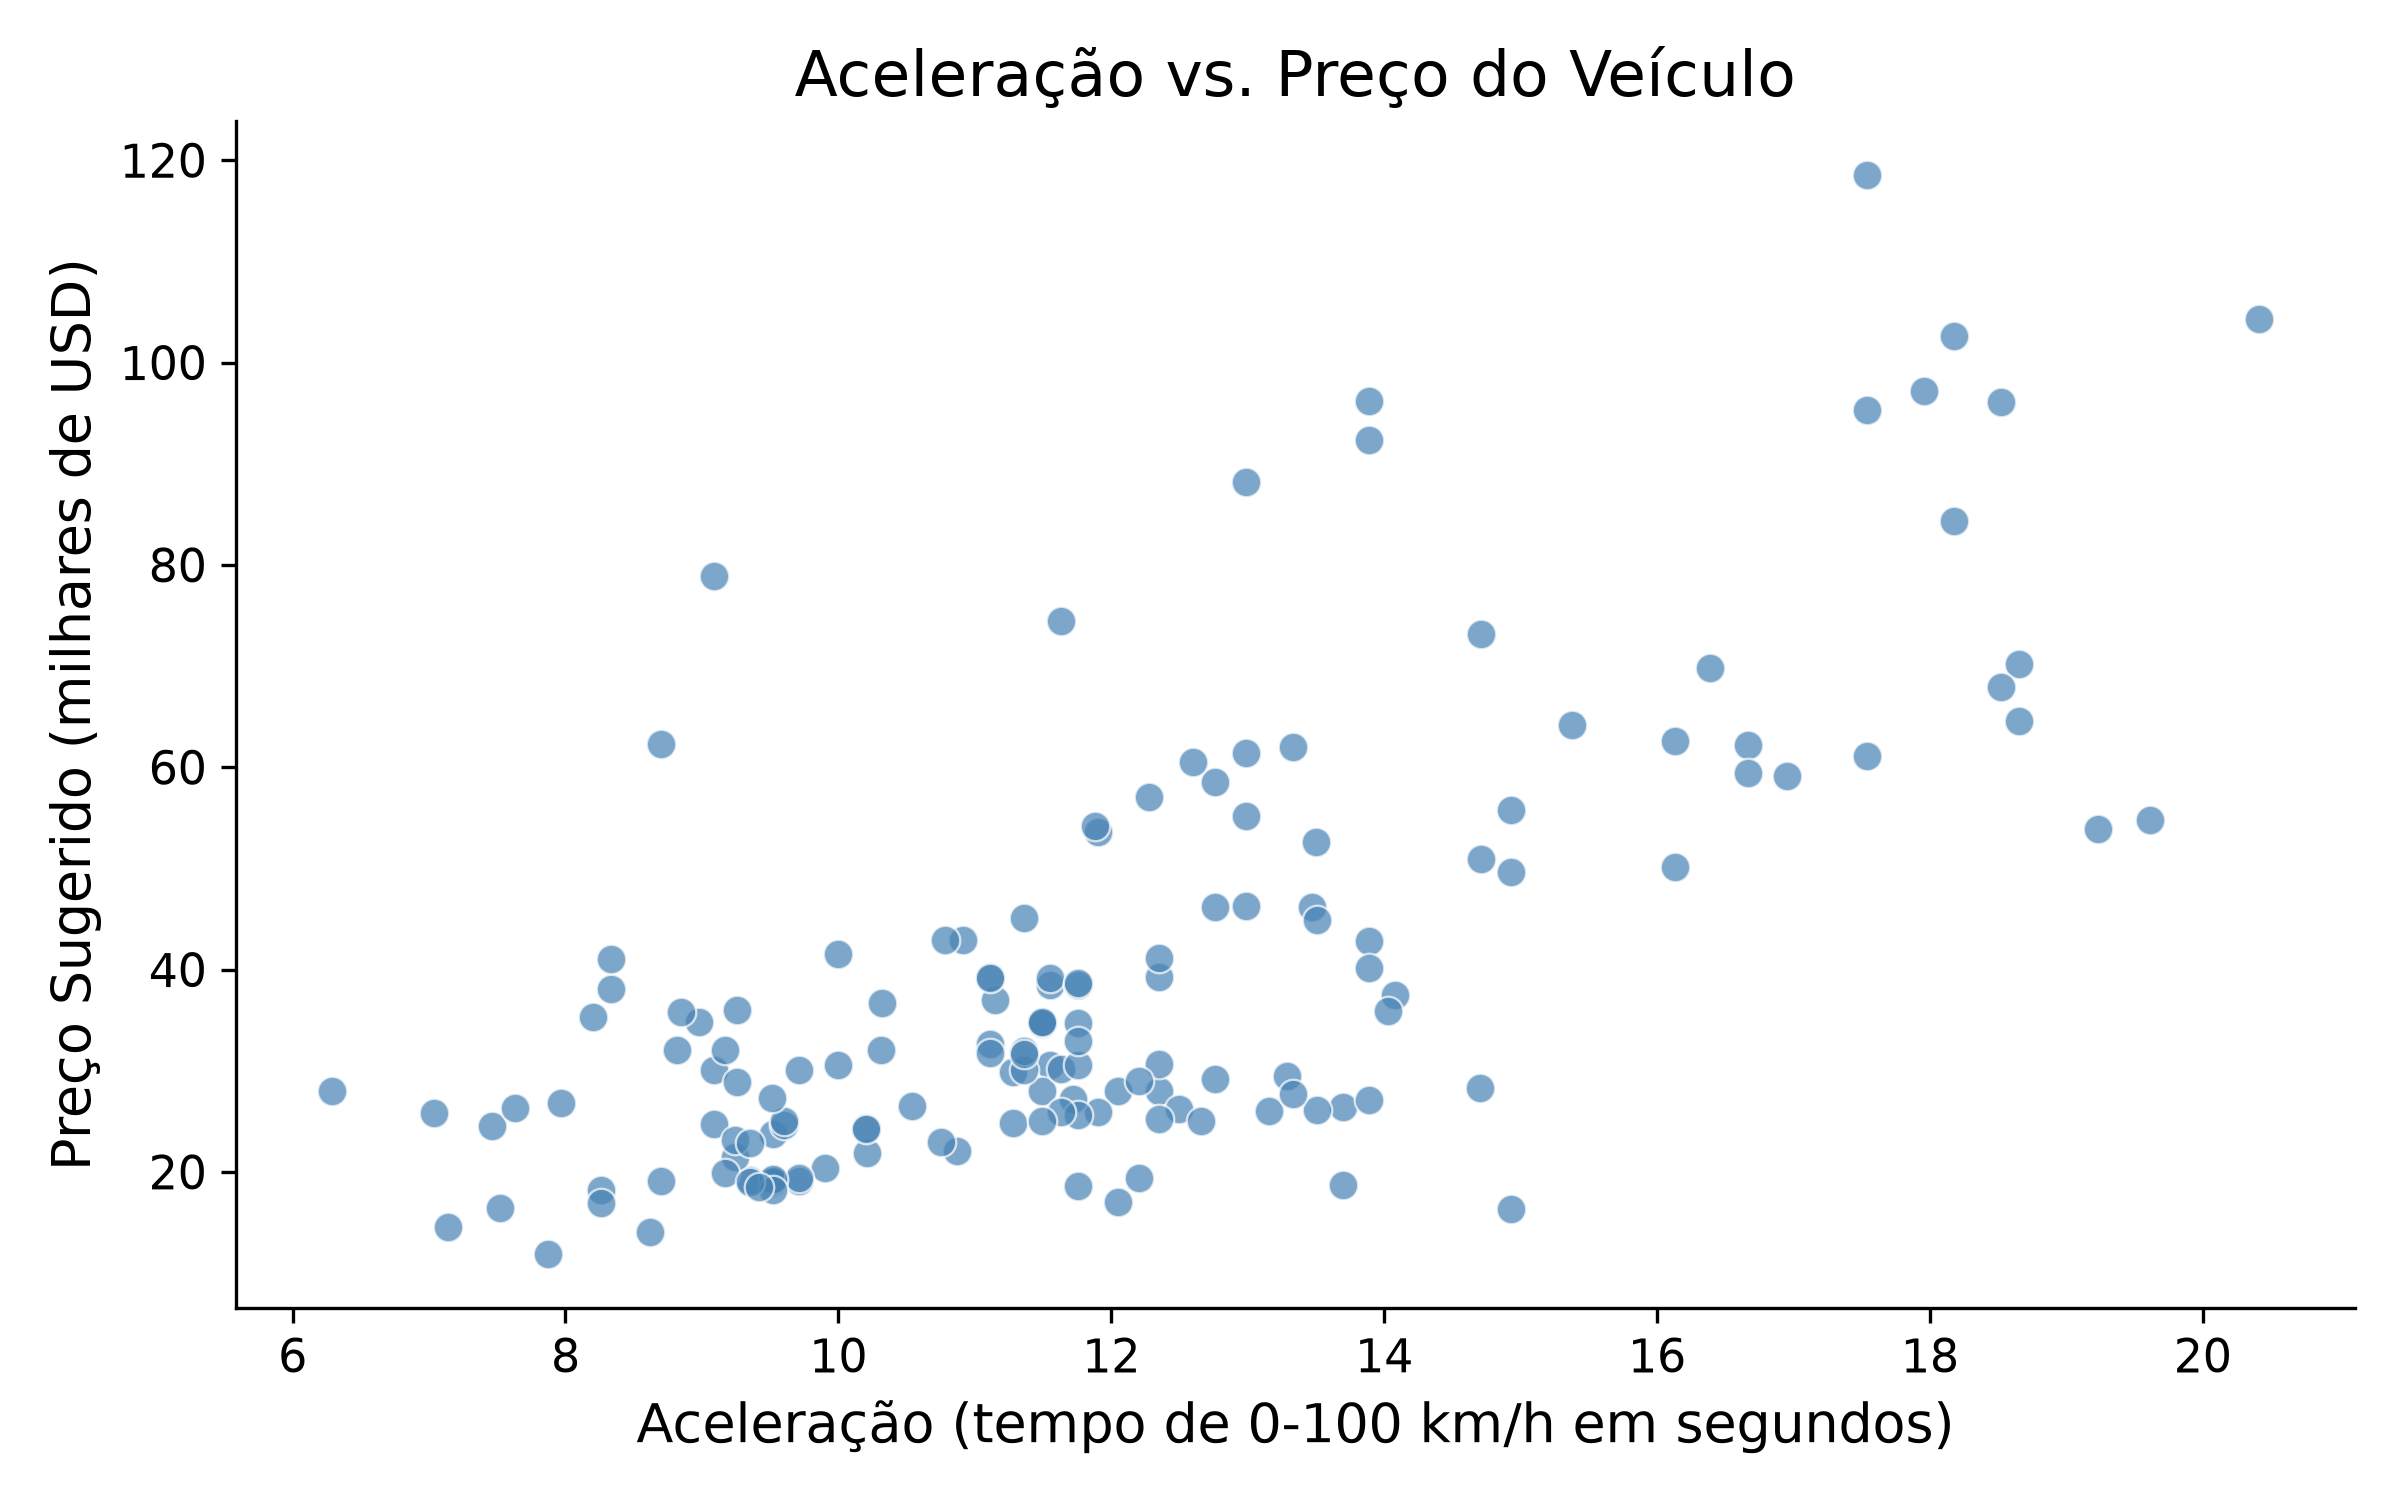
\includegraphics[width=0.95\textwidth]{car_aceleracao_vs_preco.png}
        \end{column}
    \end{columns}
\end{frame}

\begin{frame}{Correlação: Consumo vs. Aceleração}
    \begin{columns}
        \begin{column}{0.5\textwidth}
            \textbf{Consumo e Desempenho:}
            \begin{itemize}
                \item Relação negativa evidente entre o consumo (milhas por galão - mpg) e a aceleração (segundos).
                \item O comportamento dos dados sugere uma tendência não-linear.
                \item Veículos mais eficientes e econômicos (alto mpg) exigem maior tempo de aceleração.
            \end{itemize}
        \end{column}
        \begin{column}{0.5\textwidth}
            \centering
            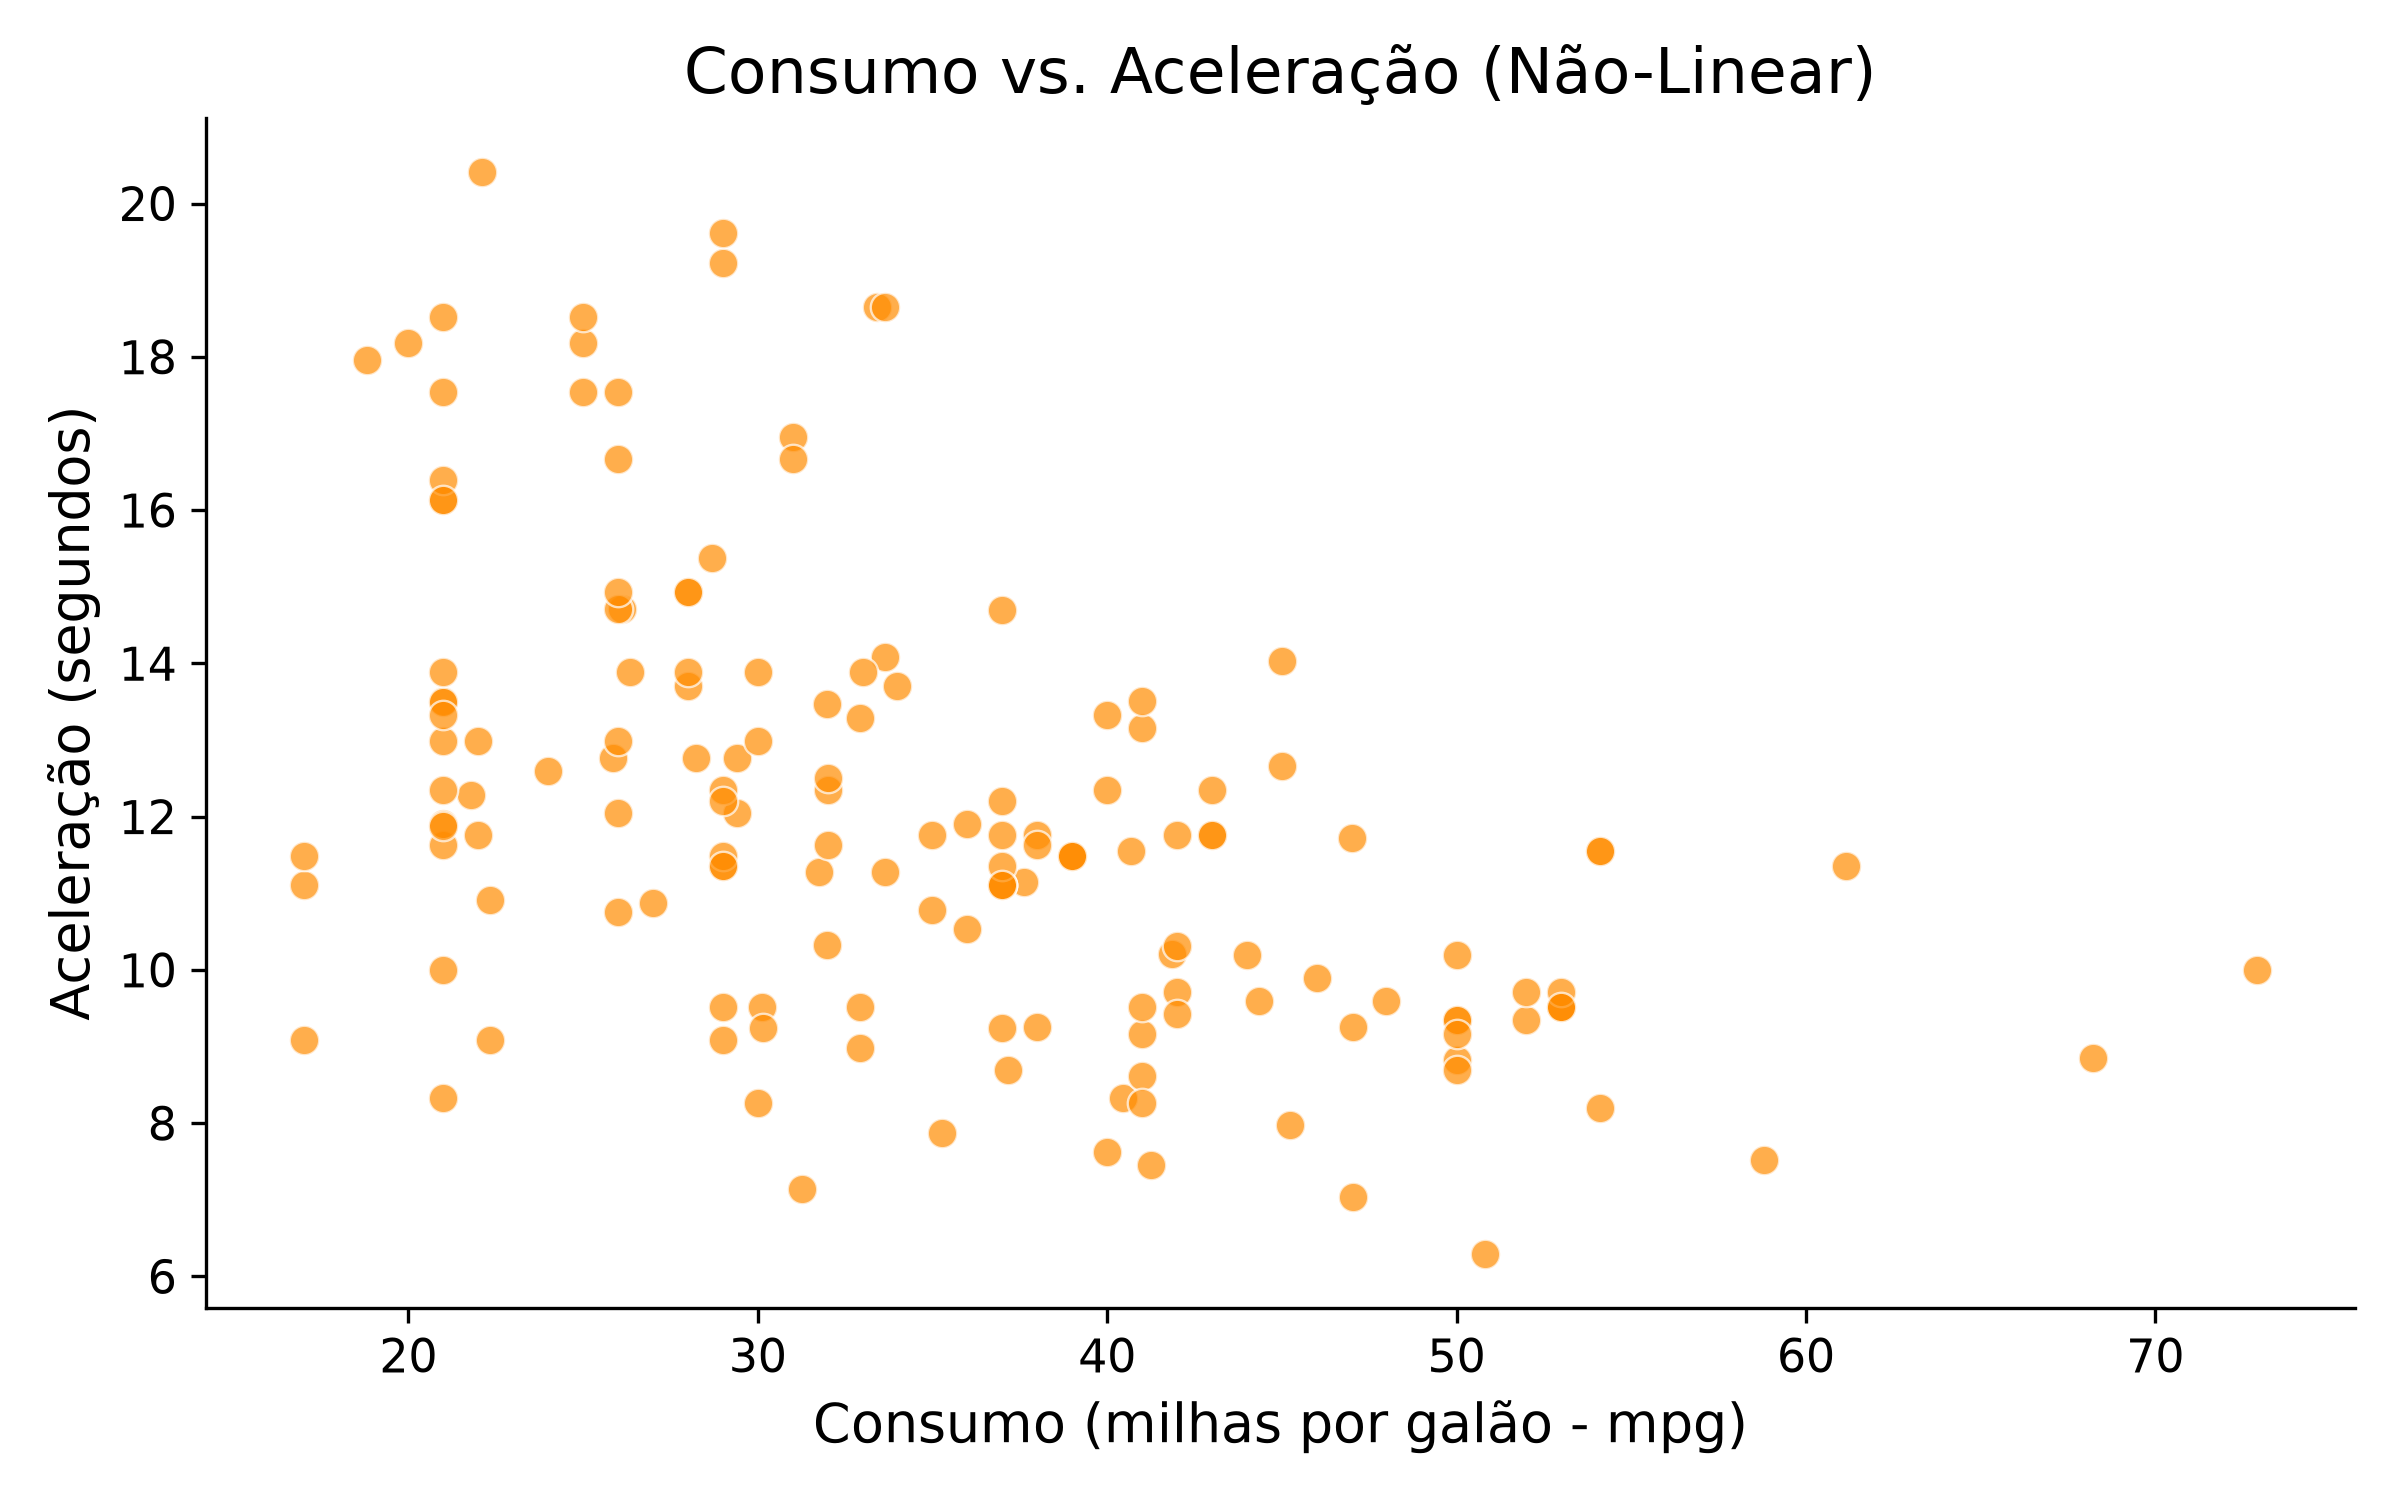
\includegraphics[width=0.95\textwidth]{car_consumo_vs_aceleracao.png}
        \end{column}
    \end{columns}
\end{frame}

\begin{frame}{Lembrando da Variância Amostral}
    \begin{itemize}
        \item A \textbf{Variância Amostral} ($s^2$) sumariza a dispersão de apenas uma variável quantitativa:
        $$s^2 = \frac{\sum_{i=1}^N (x_i - \bar{X})^2}{N - 1}$$
        \item Onde:
        \begin{itemize}
            \item $N$ é o \textbf{Tamanho da Amostra}.
            \item $\bar{X}$ é a \textbf{Média Amostral}.
            \item $x_i$ representa cada observação individual.
        \end{itemize}
        \item \textbf{Desafio:} Como podemos proceder para analisar dados bidimensionais ($X, Y$)?
        \item \textbf{Ideia:} Avaliar a dispersão conjunta das duas variáveis.
    \end{itemize}
\end{frame}

\begin{frame}{Quadrantes de Dispersão}
    \begin{columns}
        \begin{column}{0.45\textwidth}
            \begin{itemize}
                \item Ao traçar retas nos pontos correspondentes às médias amostrais $\bar{X}$ e $\bar{Y}$, dividimos o plano em quatro quadrantes.
                \item Concentração de pontos nos quadrantes 1 e 3 indica associação positiva.
                \item Concentração de pontos nos quadrantes 2 e 4 indica associação negativa.
            \end{itemize}
        \end{column}
        \begin{column}{0.55\textwidth}
            \centering
            \textbf{Quadrantes em Torno da Média}
            \vspace{0.2cm}
            \small
            \begin{tabular}{c|c}
                \textbf{Quadrante 2} & \textbf{Quadrante 1} \\
                $(x_i - \bar{X}) < 0$ & $(x_i - \bar{X}) > 0$ \\
                $(y_i - \bar{Y}) > 0$ & $(y_i - \bar{Y}) > 0$ \\
                Produto: \textbf{Negativo} & Produto: \textbf{Positivo} \\
                \hline
                \textbf{Quadrante 3} & \textbf{Quadrante 4} \\
                $(x_i - \bar{X}) < 0$ & $(x_i - \bar{X}) > 0$ \\
                $(y_i - \bar{Y}) < 0$ & $(y_i - \bar{Y}) < 0$ \\
                Produto: \textbf{Positivo} & Produto: \textbf{Negativo} \\
            \end{tabular}
        \end{column}
    \end{columns}
\end{frame}

\begin{frame}{A Covariância Amostral}
    \begin{itemize}
        \item Definimos a \textbf{Covariância Amostral} ($cov(X, Y)$) como a média dos produtos dos desvios:
        $$cov(X, Y) = \frac{\sum_{i=1}^N (x_i - \bar{X})(y_i - \bar{Y})}{N - 1}$$
        \item \textbf{Propriedades do Sinal:}
        \begin{itemize}
            \item Se $cov(X, Y) > 0$: Associação positiva (pontos nos quadrantes 1 e 3 dominam).
            \item Se $cov(X, Y) < 0$: Associação negativa (pontos nos quadrantes 2 e 4 dominam).
            \item Se $cov(X, Y) \approx 0$: Ausência de associação linear.
        \end{itemize}
        \item \textbf{Problema Crucial:} A unidade de medida da covariância é o produto das unidades dos dados originais (ex: $kg \cdot metros$), dificultando julgar a força da associação.
    \end{itemize}
\end{frame}

\begin{frame}{O Coeficiente de Correlação de Pearson ($r$)}
    \begin{itemize}
        \item Para resolver o problema de unidade, dividimos a covariância pelo produto dos desvios padrões amostrais ($s_x, s_y$):
        $$r = \frac{cov(X, Y)}{s_x \cdot s_y} = \frac{\sum_{i=1}^N (x_i - \bar{X})(y_i - \bar{Y})}{\sqrt{\sum_{i=1}^N (x_i - \bar{X})^2 \sum_{i=1}^N (y_i - \bar{Y})^2}}$$
        \item \textbf{Características de $r$:}
        \begin{itemize}
            \item É uma grandeza adimensional (sem unidade de medida).
            \item Está limitado estritamente ao intervalo: $-1 \leq r \leq 1$.
            \item $r = 1$: Relação linear positiva perfeita.
            \item $r = -1$: Relação linear negativa perfeita.
            \item $r = 0$: Sem correlação linear.
        \end{itemize}
    \end{itemize}
\end{frame}

\begin{frame}{Covariância vs. Correlação: Comparação Prática}
    \begin{itemize}
        \item A \textbf{Covariância Amostral} ($cov(X, Y)$) é sensível à escala física de cada variável.
        \item O \textbf{Coeficiente de Correlação de Pearson} ($r$) normaliza essa relação, permitindo comparar diretamente o grau de associação linear de diferentes variáveis.
    \end{itemize}
    \vspace{0.1cm}
    \centering
    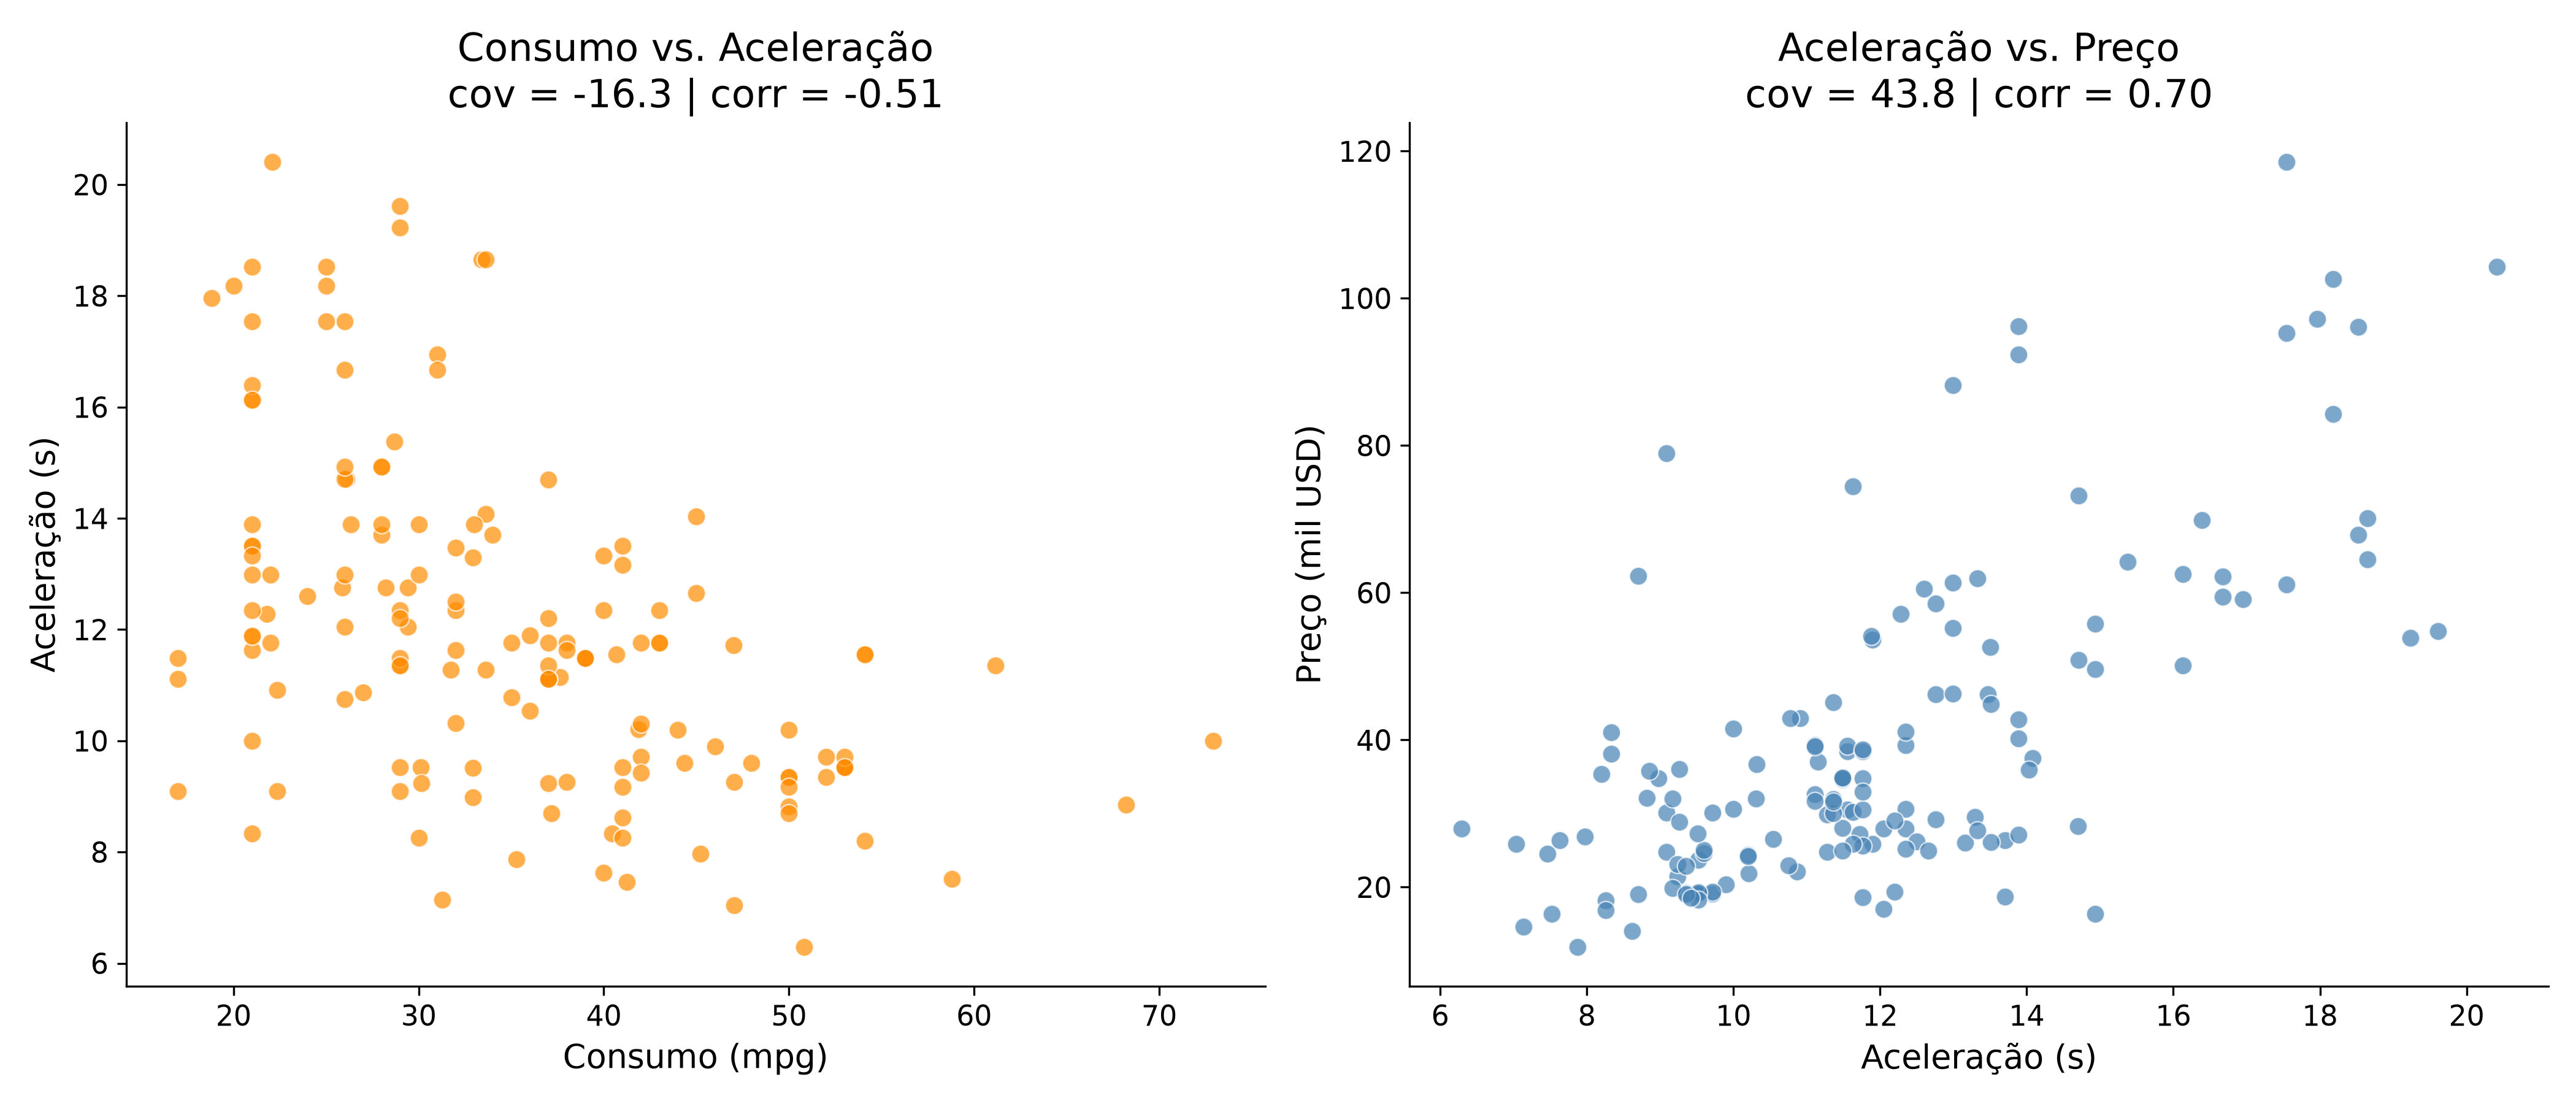
\includegraphics[width=0.9\textwidth]{car_cov_vs_corr.png}
\end{frame}

\begin{frame}{Exploração Multivariada: Plot de Pares}
    \begin{columns}
        \begin{column}{0.4\textwidth}
            \textbf{Visualização Integrada:}
            \begin{itemize}
                \item O \textbf{Plot de Pares} (Pair Plot) combina histogramas marginais na diagonal com gráficos de dispersão bivariados fora dela.
                \item Permite ao analista identificar padrões lineares, não-lineares e outliers em todas as variáveis simultaneamente.
                \item Indispensável nas etapas iniciais de exploração de dados.
            \end{itemize}
        \end{column}
        \begin{column}{0.6\textwidth}
            \centering
            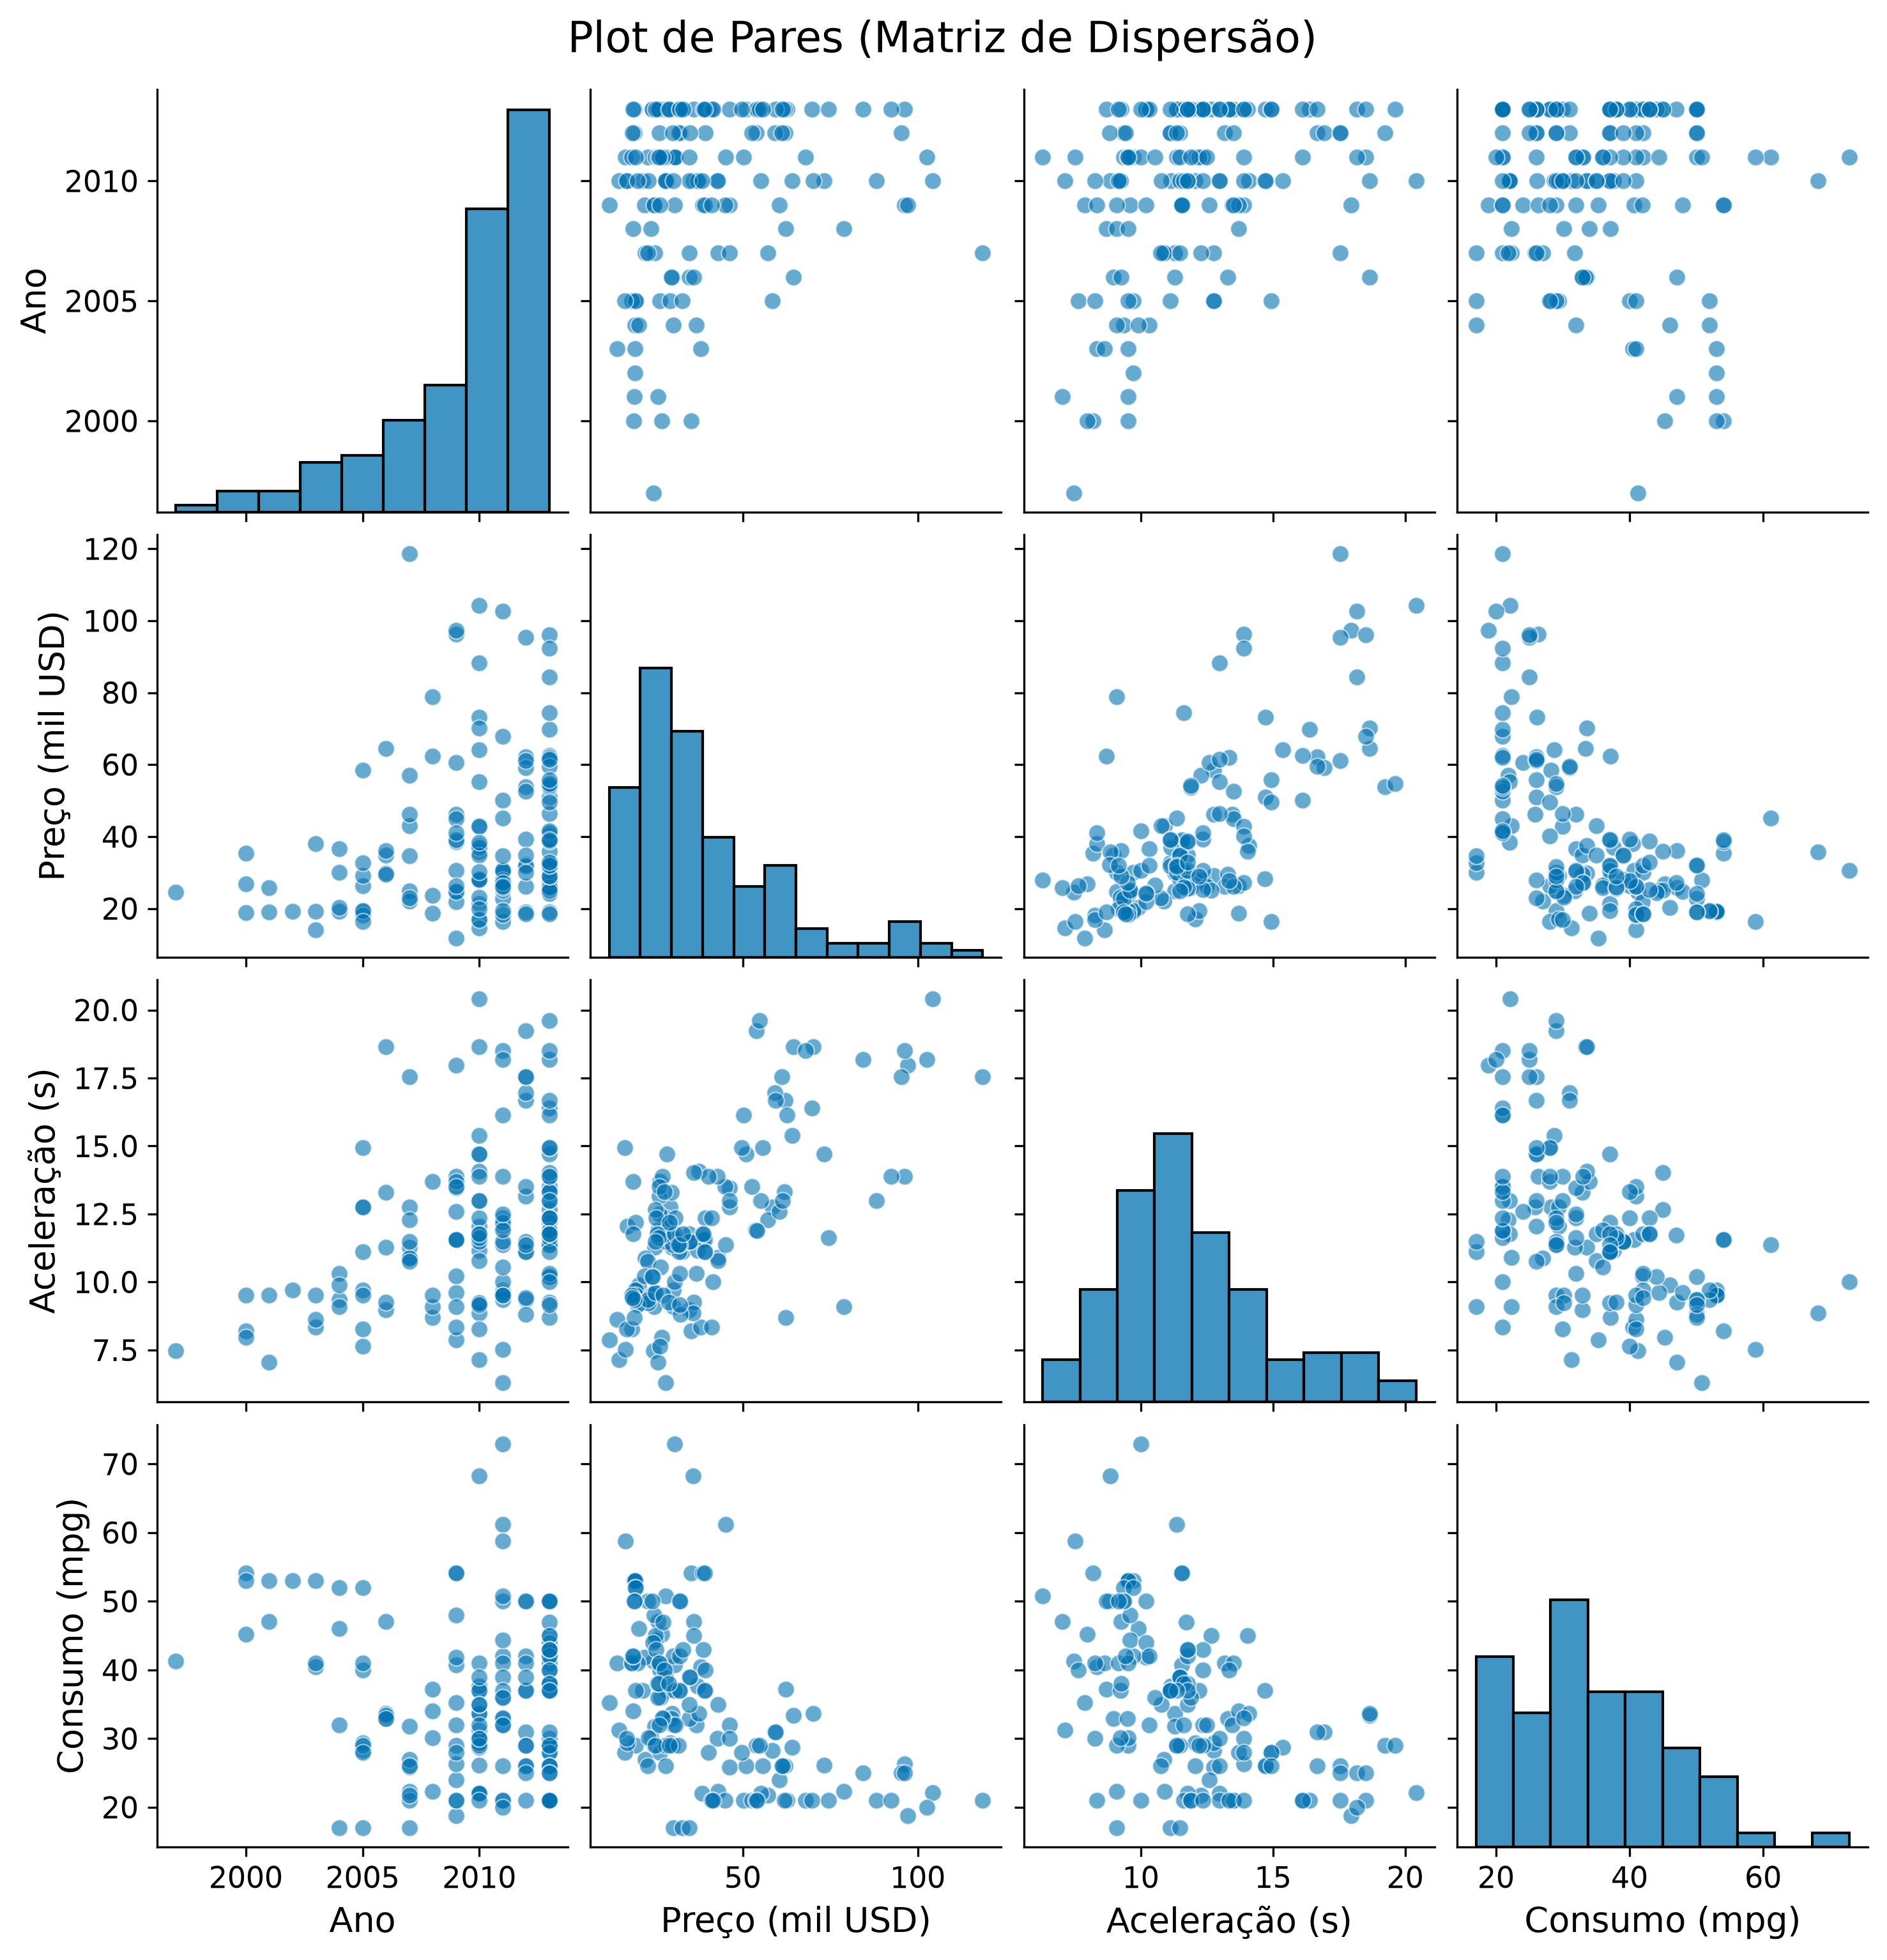
\includegraphics[width=\textwidth]{car_pairplot.png}
        \end{column}
    \end{columns}
\end{frame}

\begin{frame}{Exemplo Pareado: Passo Teórico (1/2)}
    Vamos calcular manualmente o coeficiente $r$ para o conjunto de pontos:
    $$\textbf{Dados:} \quad (1, 2), (2, 4), (3, 5), (4, 4), (5, 5)$$
    \begin{enumerate}
        \item \textbf{Médias Amostrais:}
        $$\bar{X} = \frac{1+2+3+4+5}{5} = 3.0, \quad \bar{Y} = \frac{2+4+5+4+5}{5} = 4.0$$
        \item \textbf{Desvios e Produtos:}
        \begin{itemize}
            \item $X - \bar{X} = [-2, -1, 0, 1, 2]$
            \item $Y - \bar{Y} = [-2, 0, 1, 0, 1]$
            \item Produtos dos desvios: $[4, 0, 0, 0, 2] \implies \sum = 6.0$
        \end{itemize}
        \item \textbf{Covariância Amostral:}
        $$cov(X, Y) = \frac{6.0}{5 - 1} = 1.5$$
    \end{enumerate}
\end{frame}

\begin{frame}{Exemplo Pareado: Passo Teórico (2/2)}
    $$\textbf{Dados:} \quad (1, 2), (2, 4), (3, 5), (4, 4), (5, 5)$$
    \begin{enumerate}
        \setcounter{enumi}{3}
        \item \textbf{Variâncias e Desvios Padrão Amostrais:}
        $$s_x^2 = \frac{(-2)^2 + (-1)^2 + 0^2 + 1^2 + 2^2}{4} = 2.5 \implies s_x = \sqrt{2.5} \approx 1.5811$$
        $$s_y^2 = \frac{(-2)^2 + 0^2 + 1^2 + 0^2 + 1^2}{4} = 1.5 \implies s_y = \sqrt{1.5} \approx 1.2247$$
        \item \textbf{Coeficiente de Correlação de Pearson ($r$):}
        $$r = \frac{cov(X, Y)}{s_x \cdot s_y} = \frac{1.5}{1.5811 \cdot 1.2247} = \frac{1.5}{1.9365} \approx \textbf{0.7746}$$
    \end{enumerate}
    \vspace{0.2cm}
    O resultado aponta uma associação linear positiva de moderada a forte.
\end{frame}

\begin{frame}[fragile]{Exemplo Pareado: Demonstração Computacional}
    \begin{block}{Cálculo em Python equivalente}
\begin{lstlisting}
import numpy as np
from scipy import stats

# Dados do exemplo teorico
x = np.array([1, 2, 3, 4, 5])
y = np.array([2, 4, 5, 4, 5])

# Calculo usando numpy (matriz de covariancia)
# ddof=1 garante o denominador N-1 da covariancia amostral
cov_mat = np.cov(x, y, ddof=1)
cov_xy = cov_mat[0, 1]

# Calculo de Pearson
r, p_valor = stats.pearsonr(x, y)

print(f"Covariancia Amostral: {cov_xy:.4f}")
print(f"Pearson r: {r:.4f}")
# Saida esperada:
# Covariancia Amostral: 1.5000
# Pearson r: 0.7746
\end{lstlisting}
    \end{block}
\end{frame}
